\documentclass{article}
\usepackage{graphicx}
\usepackage{url}
\usepackage{natbib}
\usepackage{todonotes}
\title{Big Literature in Climate Change}
\begin{document}
\maketitle
\begin{abstract}
Rapid increases in the number of studies published about climate change make a comprehensive assessment of the relevant literature ever more difficult. This in turn poses serious challenges for evidence-based decision making. In this paper we make the case that the challenges and opportunities presented by the explosion in relevant literature are akin to those presented by big data, and point to ways that machine learning techniques derived from big data could be applied to big literature.
\end{abstract}

\section{Introduction}
\begin{itemize}	

	\item Science policy, assessments - challenges of explosion.
    
	\item Big Literature in other sciences: \citet{Nunez-Mir2016}

	\item Canonical big data definition, 3 Vs + methods 

	\item Here, we estimate the size of the relevant literature and attempt to quantify it according to the dimensions above. This in itself is challenging due to the size of the data and requires new methods.  
\end{itemize}

\section{Estimating the Size of the Climate Literature}
% * <max.w.callaghan@gmail.com> 2017-03-23T12:44:52.581Z:
% 
% Include venn figure on WoS + Scopus & per year figure
% 
% ^.
\begin{itemize}
	\item Estimate in \citet{minx2016learning} was a lower-bound estimate because it ignored
\begin{enumerate}
	\item literature, such as grey literature not published in peer reviewed journals 
    \item literature that is not included in the Web of Science (WoS) 
    \item literature that is not directly about climate change, but that is relevant to understanding the problem and its potential solutions, such as literature on international cooperation.
\end{enumerate}

\item In this paper, we attempt a more realistic estimate of the size of the literature on climate change by
\begin{enumerate}
	\item Carrying out the same query on Scopus, and combining the results with WoS
    \item Checking the references of the literature returned by the scopus query
\end{enumerate}

\end{itemize}


\begin{figure}
%\includegraphics[width=\linewidth]{}
PLACEHOLDER
\caption{Union of Scopus and Web of Science results}
\end{figure}

\begin{figure}
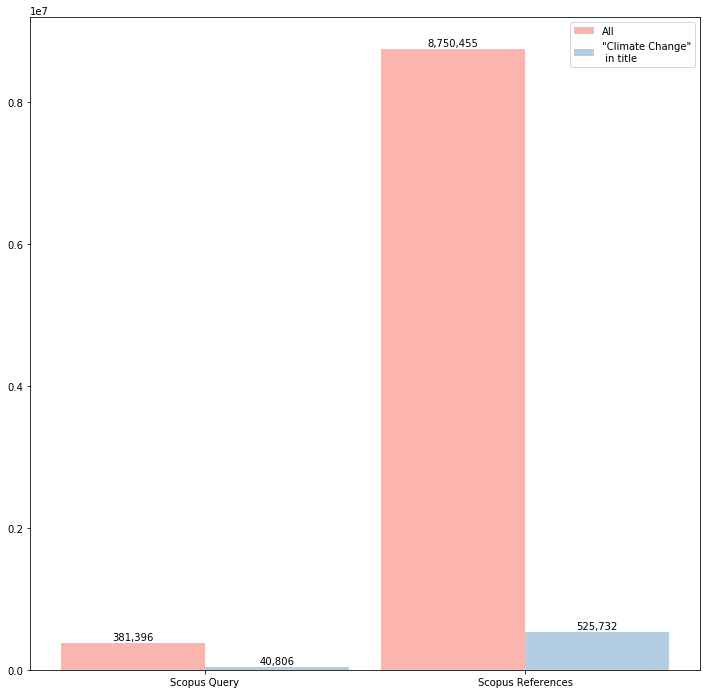
\includegraphics[width=\linewidth]{plots/scopus_docs_refs}
\caption{Number of papers retrieved from scopus, and the references contained within them}
\end{figure}


% * <max.w.callaghan@gmail.com> 2017-03-28T08:07:26.243Z:
% 
% Check for climate change in IPCC reference titles
% 
% ^.

\subsection{Dimensions of big data}
\todo{Either we show these for the whole estimate, or just wos and scopus.}
\todo{Either we address these individually, or say, in addition to volume and velocity, which we have addressed already, variety}
\begin{itemize}		
    \item Online synthesis figure as in \url{http://www.visualsedimentation.org/index.html}?
    
\end{itemize}

\subsubsection*{Volume}
\begin{itemize}
	\item Number of documents over time / number of words in titles/Abtracts?
    \item Express in GB? Reading-hours? Bibles? 
\end{itemize}

\subsubsection*{Velocity}
\begin{itemize}
	\item The papers per year figures we've made show increasing velocity, are they sufficient?
    \item What about the citation window of papers (as in the year of the earliest reference and the year of the latest)? Would this shortening be a sign the science is speeding up?
\end{itemize}


\subsubsection*{Variety}

\begin{itemize}
	\item unique words per 1000 documents and average word frequency as in Figure \ref{variety}
\end{itemize}

\begin{figure}
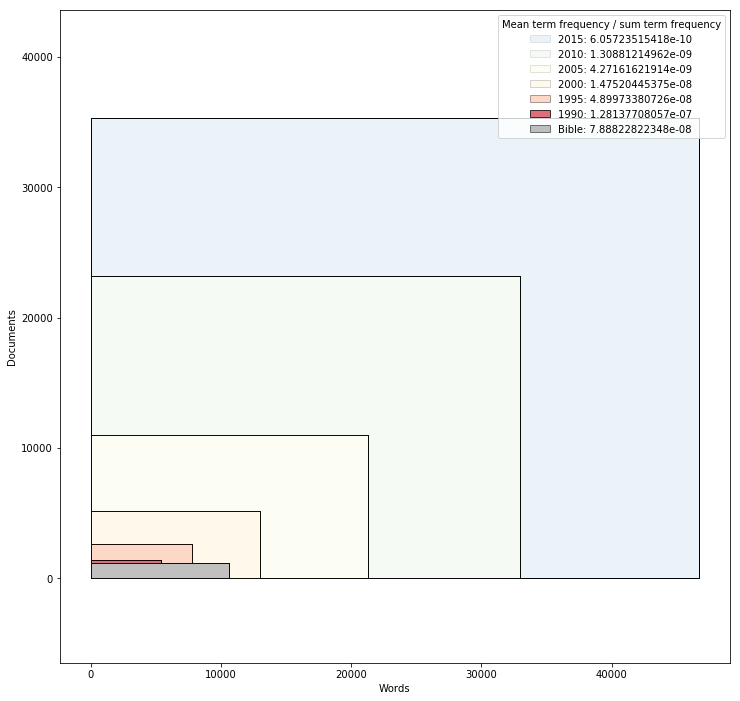
\includegraphics[width=\linewidth]{plots/volume_variety_bible}
\caption{Documents, words and average word frequency}
\label{vsquare}
\end{figure}

\begin{figure}
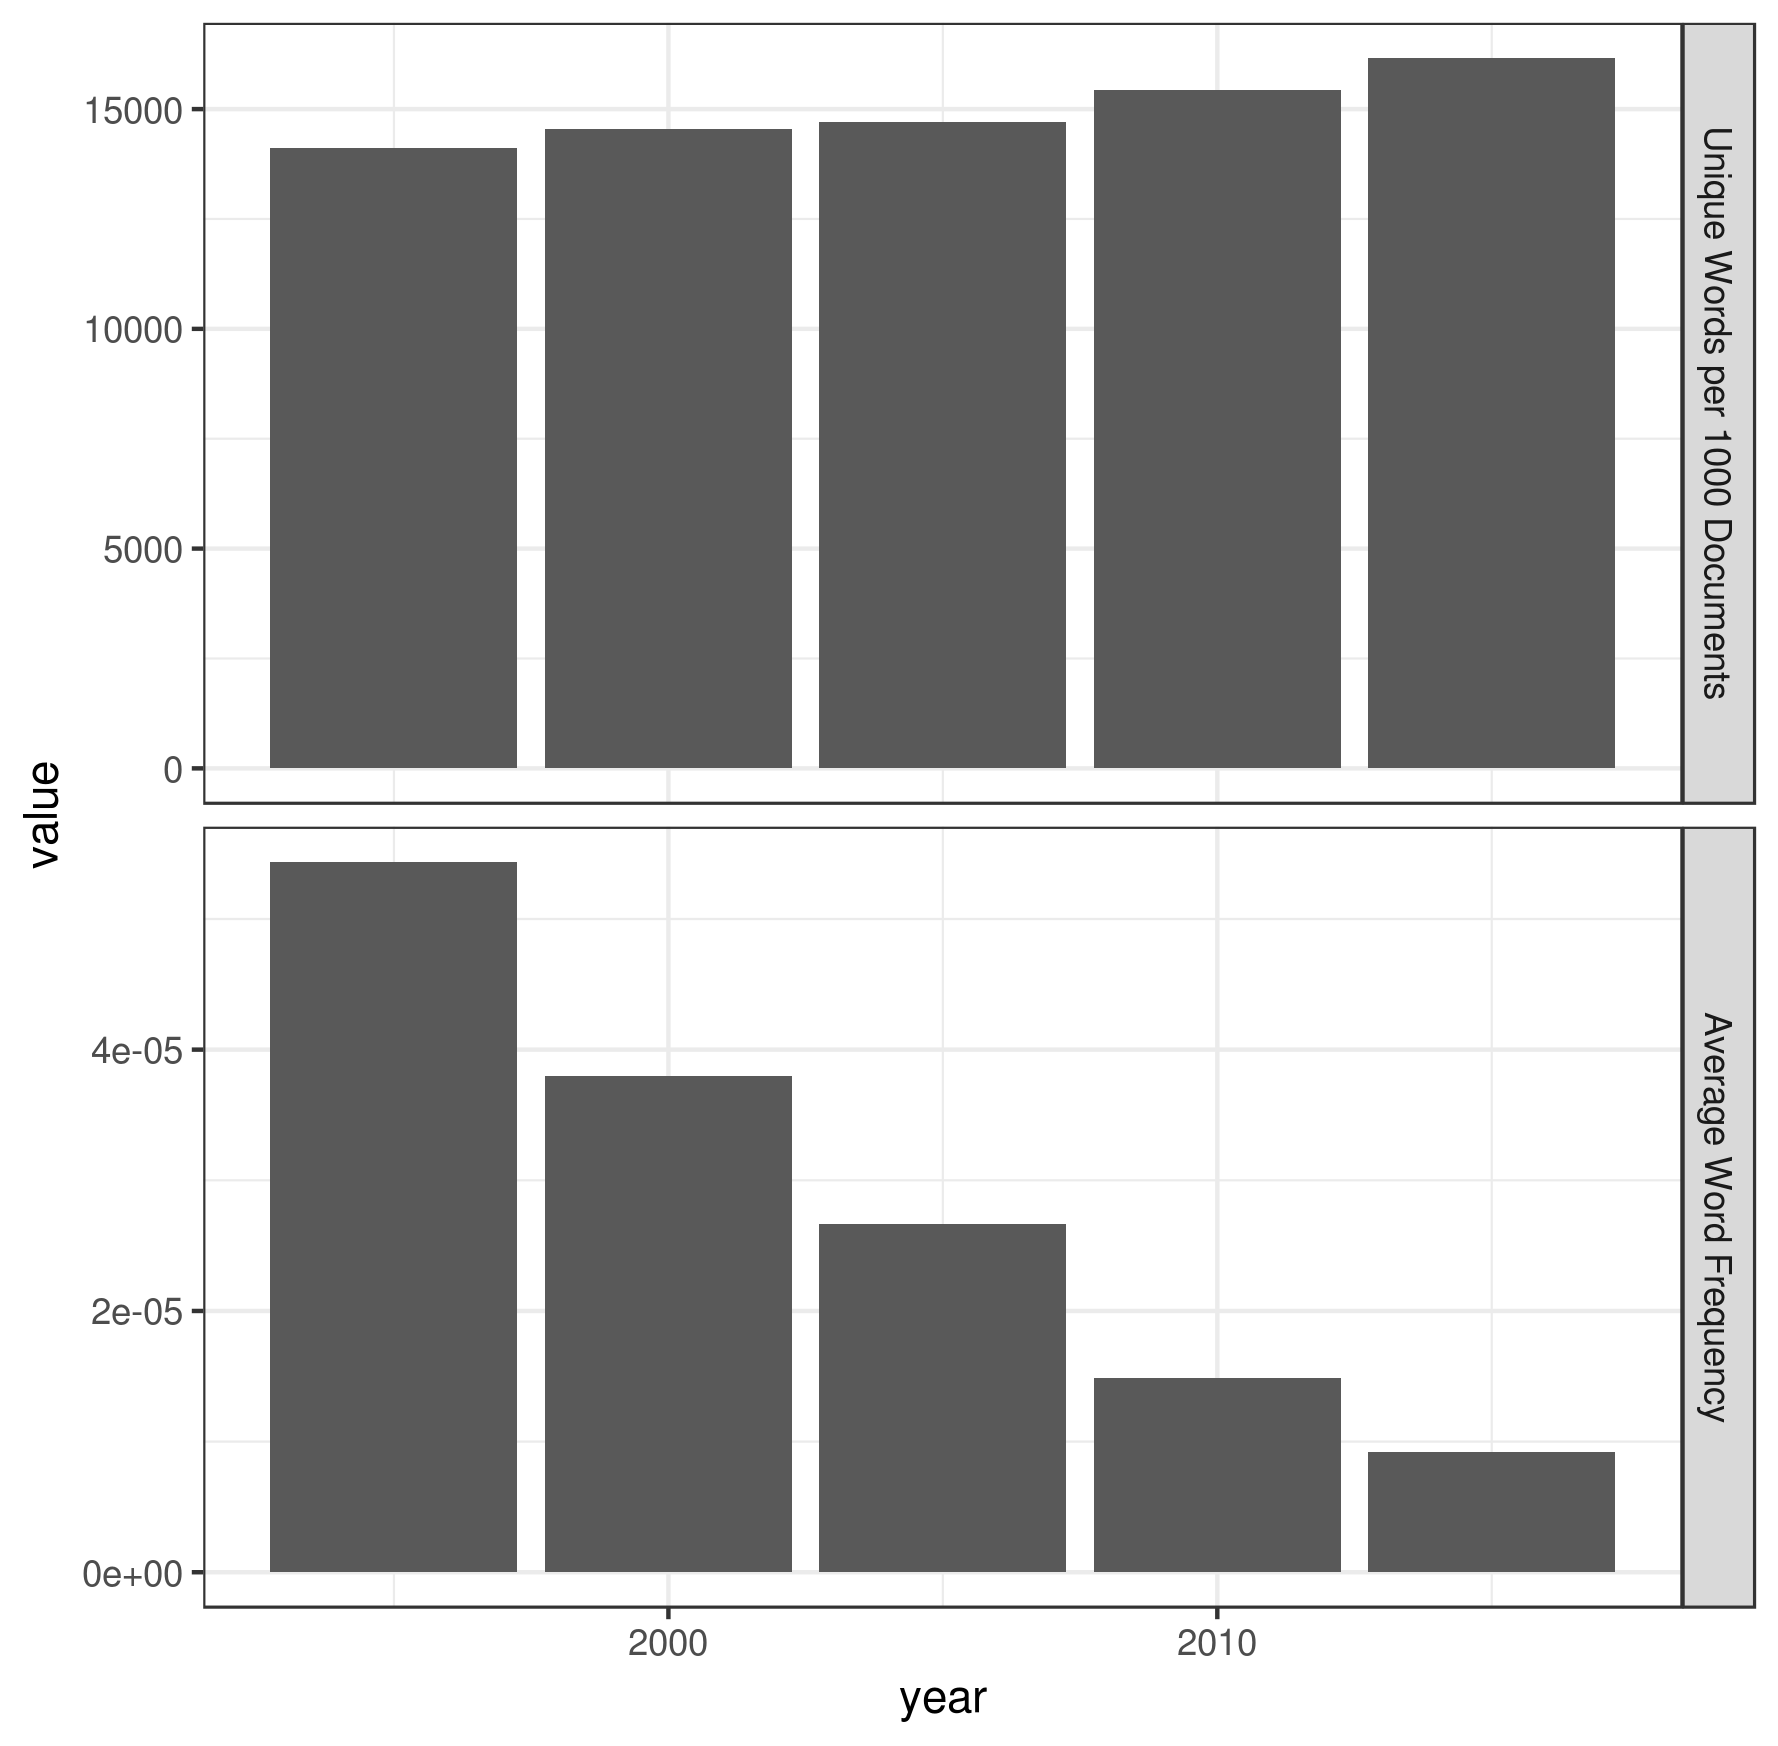
\includegraphics[width=\linewidth]{plots/variety}
\caption{Unique words per document and average word frequency [old figure from just WoS]}
\label{variety}
\end{figure}

\subsubsection*{Veracity}
Quality issues that make the simple tasks here difficult
\begin{itemize}
	\item All those missing DOIs
    \item All those different titles, different pubyears on documents with the same DOIs
    \item Author disambiguation problems
\end{itemize}
These happen because these online collections digitalise a format that was developed before digital era. Authors, references in a scientific article represent links to specific, unique objects in a way that is easy for humans to understand but very difficult for computers to understand. Like all NLP problems.

\section{Implications}
\begin{itemize}
	\item Scientific assessments cannot humanly read everything [volume]
    \item Undersampling without systematic approach results in bias [volume]
    \item Hard to keep up with fast-moving science [velocity]
    \item More variety means more topics to need expertise about [variety]
    \item Understanding the science-policy interface needs an understanding of how this big literature interacts with assessments and with policy
\end{itemize}

\section{Solutions}

\begin{itemize}
	\item Scientific assessments need systematic approach to synthesising literature with clear inclusion criteria
    \item Machine-learning, i.e. topic modelling, enabled research on science policy interface
    \item Machine-learning to aid literature synthesis
    \item Note other work in this area
    \begin{itemize}
    	\item Google already have complex and secret algorithms that decide what appears where in Google Scholar, so we can't just ignore it
        \item Other people working on using big data to ``hack'' science, e.g. \url{https://meta.com/} ``Most scientific breakthroughs have been preceded by the invention of new tools that help us see and experiment in new ways.'' 
    \end{itemize}
\end{itemize}


\listoffigures


\bibliography{Mendeley.bib}
\bibliographystyle{apalike}

\end{document}